\section{Radiovågornas frekvensindelning}

Radiospektrat omfattar frekvenser från \SI{3}{kHz} \SI{300}{GHz}. Hela frekvensområdet indelas i åtta olika delar här med sina engelska benämningar:

\begin{tabularx}{\columnwidth}{lX}
	VLF & Very Low Frequencies                  \\ 
	    & Väldigt låga frekvenser               \\
	LF  & Low Frequencies                       \\
	    & Långvåg, låga frekvenser              \\
	MF  & Medium Frequencies                    \\
	    & Mellanvåg, mellanhöga frekvenser      \\
	HF  & High Frequencies                      \\
	    & Kortvåg, höga frekvenser              \\
	VHF & Very High Frequencies                 \\
	    & Ultrakortvåg, väldigt höga frekvenser \\
	UHF & Ultra High Frequencies                \\
	    & Ultrahöga frekvenser                  \\
	SHF & Super High Frequencies                \\
	    & Superhöga frekvenser                  \\
	EHF & Extremely High Frequencies            \\
	    & Extremt höga frekvenser
\end{tabularx}

Det finns upplåtna frekvensband för radioamatörer på de flesta av dessa band och för att kalla oss radioamatörer behöver vi lära oss vilka frekvenser som gäller för oss åtminstone på de vanligaste banden. 

För att inte orsaka störningar för de som kör smalbandig telegrafi och andra smalbandiga moder så delar man ofta upp de frekvenser som sändaramatörerna får använda så att man inte skall orsaka störningar för varandra. Därför är det viktigt att lära sig ''telegrafifrekvenserna'' på banden så man inte av misstag sänder på dessa.

För den senaste utgåvan av gällande frekvensplan se SSA:s webbsida. Du ska lära dig frekvensplanen och vilka delar som är upplåtna för enbart telegrafi eller andra smalbandiga sändsningsslag för följande frekvensband: (i våglängd) \SI{160}{m}, \SI{80}{m}, \SI{40}{m}, \SI{20}{m}, \SI{17}{m}, \SI{15}{m}, \SI{12}{m}, \SI{10}{m}, \SI{6}{m}, \SI{2}{m}, \SI{70}{cm}. 

\section{Olika trafiksätt}

Detaljer om olika trafiksätt som förekommer inom amatörradio får du lära dig efter hand. Här kan KonCEPT-boken komma till god hjälp som fördjupning och vidarutbildning.

\subsection{Textöverföring}

\begin{itemize}
	\item \textbf{CW} är morsetelegrafering, sändning för hand och mottagning med hörseln. Kan även vara maskinstyrd via dator.
	\item \textbf{RTTY}, \textbf{AMTOR}, \textbf{PSK31} med flera är kommunikationssätt där tangentbord och bildskärm används vid kommunikationen (fjärrskrift).
	\item \textbf{Packet Radio} är ett kommunikationssätt där informationen grupperas i paket och radiostationerna ingår i kommunikationsnät som kan förmedla paketen över långa avstånd
	\item \textbf{Whisper} -- 
	\item \textbf{FT8} --
	\item Andra moder?
\end{itemize}

--- TODO ---

\subsection{Talöverföring}

\begin{itemize}
	\item \textbf{AM} och \textbf{SSB} är amplitudmodulerat tal, där främst SSB används på alla frekvenser från långvåg till mikrovåg.
	\item NBFM, FM med \SI{5}{kHz} deviation: Det trafiksätt som används vid FM på \SI{144}{MHz} och \SI{432}{MHz} vilket ger ca \SI{16}{kHz} bandbredd.
\end{itemize}

\emph{Att tänka på:}

Vid talöverföring på SSB använder radioamatörer av tradition alltid LSB på frekvenser under \SI{10}{MHz} och USB på frekvenser över. Anledningen har att göra med hur man i äldre apparater byggde blandare som skulle fungera på flera frekvensband. Mer om detta kan du läsa i KonCEPT-boken.

Professionella användare på kortvågen så som maritima sändarstationer och flyget använder normalt alltid USB oavsett frekvens när man använder SSB.

\subsection{Bildöverföring}

\begin{itemize}
	\item SSTV är stillbilder men räknas till TV-moder (Slow Scan Television) med så smal bandbredd att signalerna kan skickas via vanlig talkanal, t.ex. med SSB-sändare på kortvåg.
	\item ATV är amatörradioteve som är vanlig TV med hög upplösning och stor bandbredd över ibland flera MHz. Används inte på kortvåg p.g.a. sin bredbandighet utan primärt på UHF t.ex bandet  1296\,MHz.
\end{itemize}


\section{Att observera!}

När man nyttjar en amatörradiosändare måste hela den utsända signalen ligga inom amatörradiobandet. Du måste därför vara uppmärksam på både den inställda sändarfrekvensen och vilken bandbredd som ditt valda sändningsslag genererar så att du inte sänder utanför bandet.

Praktiskt kan du får sända signaler på undre sidbandet (LSB) och ha frekvensskalan inställd på \SI{3800}{kHz} därför att hela undre sidbandet då ryms inom det tillåtna spektrumet. 

Om du däremot ställer in övre sidbandet (USB) så kan du inte göra så, då kommer hela din signal i stället ligga utanför det tillåtna bandet. För att den skall rymmas inom bandet måste du minska sändarens frekvens med minst lika mycket som din högsta modulationsfrekvens och gärna ge den lite marginal. I praktiken innebär det att du aldrig bör gå närmare bandkanten än \SI{3}{kHz} och för att vara på den säkra sidan kanske du inte skall överskrida \SI{3795}{kHz} som inställd frekvens.

Du är skyldig att kunna genomföra de beräkningar som behövs och känna till tillräckligt mycket om modulationsslagen för att tillse att du inte av misstag ställer in din sändare så den sänder utanför bandet.

\emph{När det är dags för dig att själv börja sända, skaffa dig en detaljerad bandplan. Dessa kan laddas ned som PDF från SSA:s webbsida. I dag är de uppdelade i två planer, en för frekvenser till och med \SI{50}{MHz}-bandet och en för frekvensern över.}

\section{Radiovågornas frekvensindelning}

Tabellen gäller för europa (CEPT region 1).

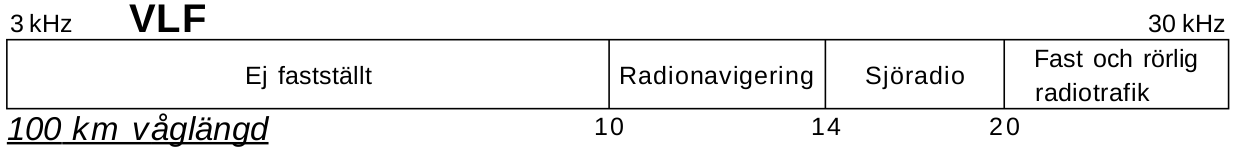
\includegraphics[width=\columnwidth]{blabok/pictures/r6-1-vlf}

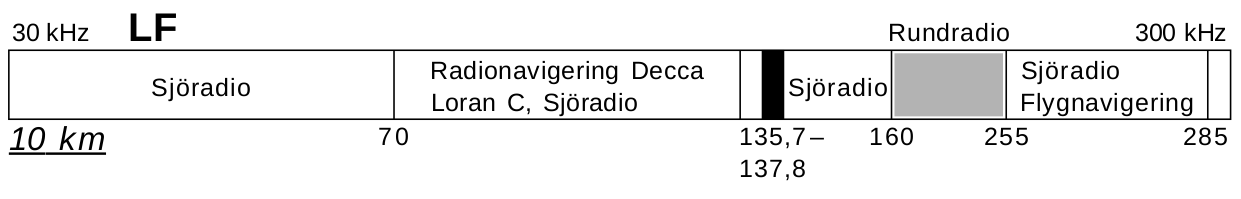
\includegraphics[width=\columnwidth]{blabok/pictures/r6-2-lf}

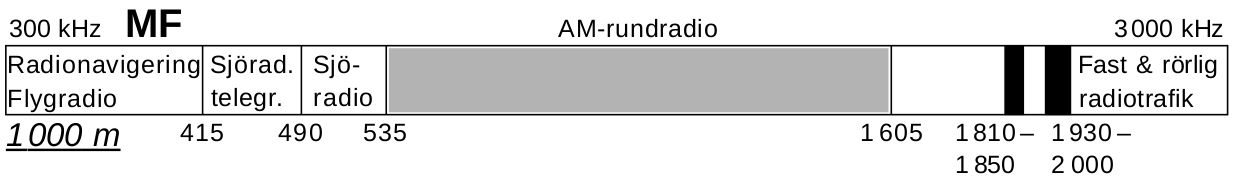
\includegraphics[width=\columnwidth]{blabok/pictures/r6-3-mf}

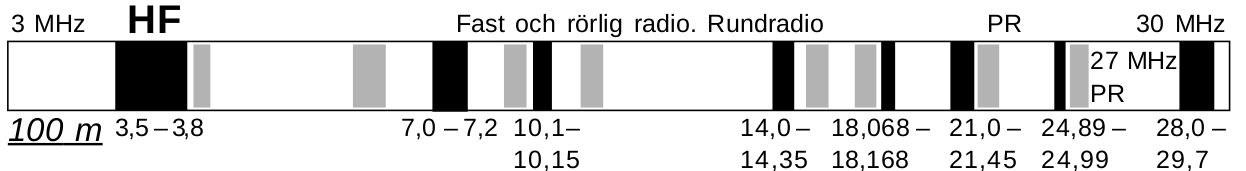
\includegraphics[width=\columnwidth]{blabok/pictures/r6-4-hf}

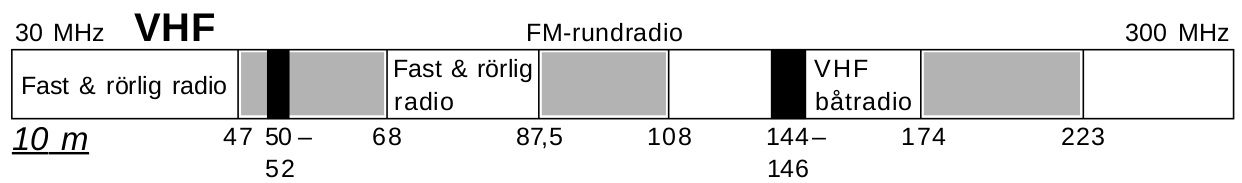
\includegraphics[width=\columnwidth]{blabok/pictures/r6-5-vhf}

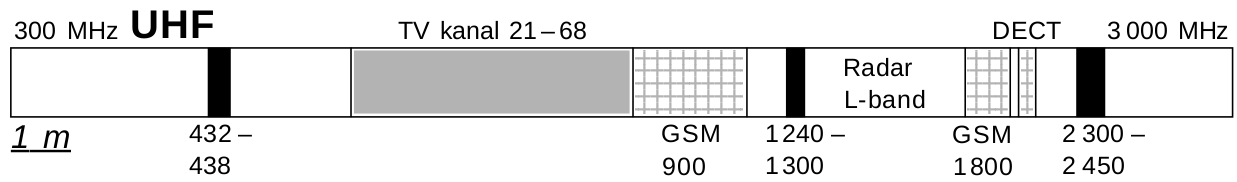
\includegraphics[width=\columnwidth]{blabok/pictures/r6-6-uhf}

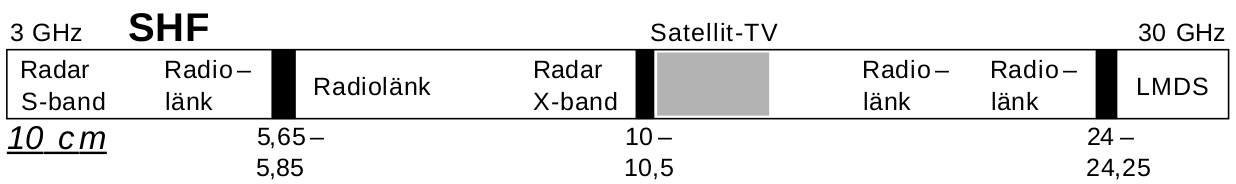
\includegraphics[width=\columnwidth]{blabok/pictures/r6-7-shf}

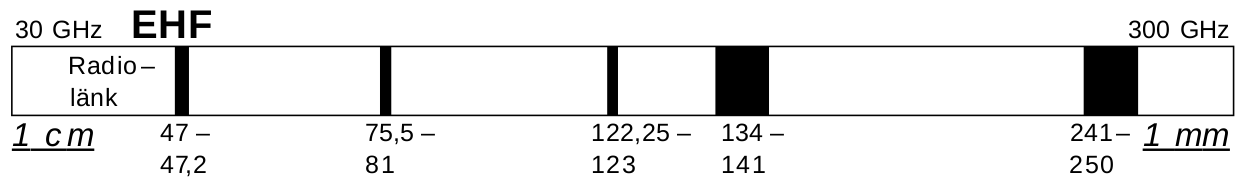
\includegraphics[width=\columnwidth]{blabok/pictures/r6-8-ehf}


\includegraphics[width=\columnwidth]{blabok/pictures/r6-9}

IARU i region 1 har gjort en detaljerad överenskommelse om hur amatörradiospektrat skall utnyttjas på bästa sätt. Detaljerade bandplaner finns att ladda hem från webbsidan ssa.se där de är översatta till sverige.

Dessa frekvensplaner uppdateras ibland så det är bra att med jämna mellanrum kontrollera om det utkommit ny utgåva och ifall det innebär att man fått ändrade användningsområden på vissa delar.

\section{Repeatertrafik}
	
I många länder finns ett system av relästationer (repeaters) runt de flesta städer.
Dessa relästationer ger dig möjlighet att, med en handapparat eller mobil radioutrustning, ha radiokontakt över ett längre avstånd. Relästationer finns bland annat på 29, 51, 145, 434 och \SI{1297}{MHz}.

Relästationen fungerar så, att det finns en infrekvens och en utfrekvens, som på
t.ex. \SI{145}{MHz} är separerad med \SI{600}{kHz}. Om man vill starta en repeater, sänder man vanligtvis en tonsignal på repeaterns infrekvens. När repeatern startar, sänder den normalt en identifiering på sin utfrekvens. 

\subsection{Bandplan för relätrafik på 29\,MHz}

\begin{tabular}{crr}
	\textbf{Kanal} & \textbf{Din RX} & \textbf{Din TX} \\
	     RH1       &    \num{29,660} &    \num{29,560} \\
	     RH2       &    \num{29,670} &    \num{29,570} \\
	     RH3       &    \num{29,680} &    \num{29,580} \\
	     RH4       &    \num{29,680} &    \num{29,590}
\end{tabular}

\subsection{Bandplan för relätrafik på 50\,MHz}

\begin{tabular}{crr}
	\textbf{Kanal} & \textbf{Din RX} & \textbf{Din TX} \\
	     RF81      &    \num{51,810} &    \num{51,210} \\
	     RF83      &    \num{51,830} &    \num{51,230} \\
	     RF85      &    \num{51,850} &    \num{51,250} \\
	     RF87      &    \num{51,870} &    \num{51,270} \\
	     RF89      &    \num{51,890} &    \num{51,290} \\
	     RF91      &    \num{51,910} &    \num{51,310} \\
	     RF93      &    \num{51,930} &    \num{51,330} \\
	     RF95      &    \num{51,950} &    \num{51,350} \\
	     RF97      &    \num{51,970} &    \num{51,370} \\
	     RF99      &    \num{51,990} &    \num{51,390}
\end{tabular}
	
\subsection{Bandplan för relätrafik på 145\,MHz}

I dag används en indelning av kanalerna om 12,5\,kHz på 145\,MHz medan man tidigare körde 25\,kHz kanalindelning. Jag har valt att även ta med de gamla beteckningarna eftersom de än i dag är vanligare att de används i dagligt tal.

För provet är det dock de nya kanalbenämningarna som man behöver kunna.

\begin{tabular}{llrr}
	\textbf{Kanal} & \textbf{f.d.} & \textbf{Din RX} & \textbf{Din TX} \\
	RV48           & RØ            &        145,6000 &        145,0000 \\
	RV49           & RØX           &        145,6125 &        145,0125 \\
	RV50           & R1            &        145,6250 &        145,0250 \\
	RV51           & R1X           &        145,6375 &        145,0375 \\
	RV52           & R2            &        145,6500 &        145,0500 \\
	RV53           & R2X           &        145,6625 &        145,0625 \\
	RV54           & R3            &        145,6750 &        145,0750 \\
	RV55           & R3X           &        145,6875 &        145,0875 \\
	RV56           & R4            &        145,7000 &        145,1000 \\
	RV57           & R4X           &        145,7125 &        145,1125 \\
	RV58           & R5            &        145,7250 &        145,1250 \\
	RV59           & R5x           &        145,7375 &        145,1375 \\
	RV60           & R6            &        145,7500 &        145,1500 \\
	RV61           & R6X           &        145,7625 &        145,1625 \\
	RV62           & R7            &        145,7750 &        145,1750 \\
	RV63           & R7X           &        145,7875 &        145,1875
\end{tabular}





\subsection{Bandplan för relätrafik på 434\,MHz}

I dag används kanalindelning om \SI{12,5}{kHz} i stället för som tidigare \SI{25}{kHz} och ännu längre tillbaka i tiden när man även tillät \SI{75}{kHz} breda kanaler.

För amatörradioprovet ska man kunna frekvenserna för den nya kanalnumreringen. I dagligt tal används fortfarande de gamla benämningarna (RU3X) så de finns också med.


% Flyttad hit av layoutskäl

\vspace{1em} \hrule \vspace{1em}

\emph{Kom ihåg:}

\begin{itemize}
	\item Avståndet mellan en repeaters in- och utfrekvens!
	\begin{itemize}
		\item På 29\,MHz är avståndet 100\,kHz
		\item På 51\,MHz är avståndet 600\,kHz
		\item På 145\,MHz är avståndet 600\,kHz
		\item På 434\,MHz är avståndet \SI{2000}{kHz}
		\item På \SI{1296}{MHz} är avståndet \SI{6000}{kHz}
	\end{itemize}
	\item Hela den utsända signalen måste rymmas inom bandgränserna för amatörradio när du sänder.
\end{itemize}

\emph{Lär dig:}

\begin{itemize}
	\item Vilka frekvenser som används inom amatörradio
	\item Bandplanerna och vilken del som är upplåten enbart för CW
	\item Kunna räkna fram frekvenser för repeatrar på olika band. Tips lär dig duplexavstånd, kanalavstånd och första kanalnamnet på respektive band så kan du räkna fram det.
	\item Att vid SSB-trafik används LSB under \SI{10}{MHz} och USB på frekvenser över \SI{10}{MHz}
\end{itemize}

\vspace{1em} \hrule \vspace{1em}



\begin{tabular}{llrr}
	\textbf{Kanal} & \textbf{f.d.} & \textbf{Din RX} & \textbf{Din TX} \\
	RU368          & RU0           &        434,6000 &        432,6000 \\
	RU369          & RU0X          &        434,6125 &        432,6125 \\
	RU370          & RU1           &        434,6250 &        432,6250 \\
	RU371          & RU1X          &        434,6375 &        432,6375 \\
	RU372          & RU2           &        434,6500 &        432,6500 \\
	RU373          & RU2X          &        434,6625 &        432,6625 \\
	RU374          & RU3           &        434,6750 &        432,6750 \\
	RU375          & RU3X          &        434,6875 &        432,6875 \\
	RU376          & RU4           &        434,7000 &        432,7000 \\
	RU377          & RU4X          &        434,7125 &        432,7125 \\
	RU378          & RU5           &        434,7250 &        432,7250 \\
	RU379          & RU5X          &        434,7375 &        432,7375 \\
	RU380          & RU6           &        434,7500 &        432,7500 \\
	RU381          & RU6X          &        434,7625 &        432,7625 \\
	RU382          & RU7           &        434,7750 &        432,7750 \\
	RU383          & RU7X          &        434,7875 &        432,7875 \\
	RU384          & RU8           &        434,8000 &        432,8000 \\
	RU385          & RU8X          &        434,8125 &        432,8125 \\
	RU386          & RU9           &        434,8250 &        432,8250 \\
	RU387          & RU9X          &        434,8375 &        432,8375 \\
	RU388          & RU10          &        434,8500 &        432,8500 \\
	RU389          & RU10X         &        434,8625 &        432,8625 \\
	RU390          & RU11          &        434,8750 &        432,8750 \\
	RU391          & RU11X         &        434,8875 &        432,8875 \\
	RU392          & RU12          &        434,9000 &        432,9000 \\
	RU393          & RU12X         &        434,9125 &        432,9125 \\
	RU394          & RU13          &        434,9250 &        432,9250 \\
	RU395          & RU13X         &        434,9375 &        432,9375 \\
	RU396          & RU14          &        434,9500 &        432,9500 \\
	RU397          & RU14X         &        434,9625 &        432,9625 \\
	RU398          & RU15          &        434,9750 &        432,9750 \\
	RU399          & RU15X         &        434,9875 &        432,9875
\end{tabular}

\subsection{Bandplan för relätrafik på 1297\,MHz}

\begin{tabular}{lrr}
	\textbf{Kanal} & \textbf{Din RX} & \textbf{Din TX} \\
	RM0            &        1297,000 &        1291,000 \\
	RM1            &        1297,025 &        1291,025 \\
	RM2            &        1297,050 &        1291,050 \\
	RM3            &        1297,075 &        1291,075 \\
	RM4            &        1297,100 &        1291,100 \\
	RM5            &        1297,125 &        1291,125 \\
	RM6            &        1297,150 &        1291,150 \\
	RM7            &        1297,175 &        1291,175 \\
	RM8            &        1297,200 &        1291,200 \\
	RM9            &        1297,225 &        1291,225 \\
	RM10           &        1297,250 &        1291,250 \\
	RM11           &        1297,275 &        1291,275 \\
	RM12           &        1297,300 &        1291,300 \\
	RM13           &        1297,325 &        1291,325 \\
	RM14           &        1297,350 &        1291,350 \\
	RM15           &        1297,375 &        1291,375 \\
	RM16           &        1297,400 &        1291,400 \\
	RM17           &        1297,425 &        1291,425 \\
	RM18           &        1297,450 &        1291,450 \\
	RM19           &        1297,475 &        1291,475
\end{tabular}


